
\documentclass[a4paper,UKenglish,cleveref, autoref, thm-restate]{lipics-v2021}
%This is a template for producing LIPIcs articles. 
%See lipics-v2021-authors-guidelines.pdf for further information.
%for A4 paper format use option "a4paper", for US-letter use option "letterpaper"
%for british hyphenation rules use option "UKenglish", for american hyphenation rules use option "USenglish"
%for section-numbered lemmas etc., use "numberwithinsect"
%for enabling cleveref support, use "cleveref"
%for enabling autoref support, use "autoref"
%for anonymousing the authors (e.g. for double-blind review), add "anonymous"
%for enabling thm-restate support, use "thm-restate"
%for enabling a two-column layout for the author/affilation part (only applicable for > 6 authors), use "authorcolumns"
%for producing a PDF according the PDF/A standard, add "pdfa"

%\pdfoutput=1 %uncomment to ensure pdflatex processing (mandatatory e.g. to submit to arXiv)
%\hideLIPIcs  %uncomment to remove references to LIPIcs series (logo, DOI, ...), e.g. when preparing a pre-final version to be uploaded to arXiv or another public repository

%\graphicspath{{./graphics/}}%helpful if your graphic files are in another directory

\bibliographystyle{plainurl}% the mandatory bibstyle

\title{Advanced Data Structures: Final Report}

\author{Robert Krause}{Matrikelnummer: 2116165}{uflfu@student.kit.edu}{}{}

\authorrunning{R. Krause}

\Copyright{Robert Krause}

\ccsdesc[100]{\textcolor{red}{Replace ccsdesc macro with valid one}} %TODO mandatory: Please choose ACM 2012 classifications from https://dl.acm.org/ccs/ccs_flat.cfm 

\keywords{Predecessor, Range Minimum Queries}

\category{} %optional, e.g. invited paper

\relatedversion{}


%\nolinenumbers %uncomment to disable line numbering



%Editor-only macros:: begin (do not touch as author)%%%%%%%%%%%%%%%%%%%%%%%%%%%%%%%%%%
\EventEditors{John Q. Open and Joan R. Access}
\EventNoEds{2}
\EventLongTitle{42nd Conference on Very Important Topics (CVIT 2016)}
\EventShortTitle{CVIT 2016}
\EventAcronym{CVIT}
\EventYear{2016}
\EventDate{December 24--27, 2016}
\EventLocation{Little Whinging, United Kingdom}
\EventLogo{}
\SeriesVolume{42}
\ArticleNo{23}
%%%%%%%%%%%%%%%%%%%%%%%%%%%%%%%%%%%%%%%%%%%%%%%%%%%%%%

\begin{document}

\maketitle

\section{Introduction}
The first part of the task was to implement a predecessor data structure. More specifically we are given a 
input of $n$ numbers sorted in ascending order and a list of $q$ queries. Given Integer $x$ as query, it 
should return the largest Integer in $A$ which is smaller or equal to $x$. I chose to implement y-Fast-Tries, 
because it originally is a dynamic data structure. Since we are given a static inputs I was curious to try 
and make some adjustments to improve performance and memory requirements for the static case.\\
The second part of the assignment was to implement three data structures for range minimum queries. In this 
case we are given a list of $n$ numbers $A$ in no particular order and a list of tuples $(s,e)$ as queries. 
For a given query $(s,e)$ the result should be the index of the smallest element between index $s$ and $e$. 
I implemented a naive data structure requiring $\mathcal{O}(n^2)$ space, one using $\mathcal{O}(nlogn)$ 
space and a final one using linear space.\\
Additional requirements were that the largest possible input could be represented by a 64-bit unsigned 
Integer.

\section{Algorithms and Data Structures}
\subsection{Range Minimum Queries}
\paragraph*{x-Fast-Trie} The x-Fast-Trie is a binary tree data structure where values are represented as leaves. Each sub-tree 
stores the values with a common prefix in the binary representation. Inner nodes therefore represent a 
specific prefix and are only stored if they have leaves in their sub-tree. Because of this, the height of 
the tree is dependent on the length of the binary representation of the input. In our case the longest 
input could be up to $W=$64 Bits. I decided to make the height of the tree dynamic by looking at the largest 
actual input. This way if only the largest input would be $2^{32} - 1$ the height of the tree $W$ would be only 
32 instead of 64, saving memory and runtime. The nodes are stored in hash tables for each level of the tree 
with their binary-prefix as key. This allows us to find each node in constant time, given its prefix. 
Additionally each inner node stores the index in the input of the largest leaf to the left and the smallest 
leaf to the right, we call them descendant indexes. The leaves do not have to store pointers to the 
predecessor and successor, since we can just increment the index.
We can then perform a predecessor query on this data structure by using binary search on the levels by bit-
shifting the input to get the binary-prefix as key into the hash tables. This is logarithmic in the height 
of the tree. If the resulting node is not a leaf we can use the descendant index to the max left to get our 
result. If it is not set we can go to the min right and decrement the index by one to get the result. The 
required memory is $\mathcal{O}(Wn)$ and runtime is in $\mathcal{O}(logW)$ for perfect hashing or expected $\mathcal{O}(logW)$ for a regular hash table respectively. 

\paragraph*{y-Fast-Trie} The y-Fast-Trie uses a two level approach to reduce the memory requirements of the x-Fast-Trie while 
maintaining asymptotic runtime. To achieve this we again calculate the $W$ based on the largest input. Then 
we split the input into blocks of size $W$ and choose the minimum of each block as representative. These 
representatives are stored in a x-Fast-Trie. A predecessor query is done in two steps, first the block 
number has to be identified. This is done by querying the x-Fast-Trie for the index of the predecessor 
instead of the predecessor itself. After that we have to search for the predecessor in the block. This is 
done using binary search instead of using a binary tree, since, for our static case, we do not need the 
improved insert performance of a binary tree. The required memory is reduced to $\mathcal{O}(n)$.
\subsection{Predecessor}
\paragraph*{Naive} The naive solution ranged minimum queries stores the solution to all possible $n^2$ queries. By only 
storing the solutions for queries $(s,e)$ where $s \leq e$ we can reduce the memory consumption by half. A 
range minimum query becomes two table look-ups because solutions are stored in a two-dimensional vector. 
Initialization takes time $\mathcal{O}(n^2)$ using dynamic programming.

\paragraph*{$\mathcal{O}(nlogn)$ space} The idea of this data structure is to only store solutions to queries of the type $(s, s+2^k-1)$. This way 
the memory requirements decrease to $\mathcal{O}(nlogn)$ space. A query $(s, e)$ consists of two sub-
queries $(s, s+2^l-1)$ and $(e-2^l+1, e)$ which in turn each are made up of two table look-ups. Finally the 
result is the argmin of sub-query results. The data-structure is initialized via dynamic programming, by 
iterating over the lengths of queries $l$ in the outer loop and over the query-starts $s$ in the inner 
loop. By storing the solutions in a two-dimensional vector $M[l][x]$ instead of $M[x][l]$ we can improve 
cache usage.

\paragraph*{Linear Space} To improve upon the previous data structure we again split the input into blocks of size $s = logn/4$. For 
each block we store the position of its minimum in a vector $B'$ and the minimums are store in the $nlogn$-
data structure from above. Each query then consists of up to three queries one query spanning all blocks 
which are fully contained in the query (using nlogn-data structure) and up to two queries additional 
queries, one for the partial starting and one partial ending block respectively. To get constant query time 
for the partial queries we need to store all possible solutions for each of the blocks. Using cartesian 
trees we can identify blocks for which all queries would have the same result. This way we avoid storing 
redundant solution patterns and keep the $\mathcal{O}(n)$ memory requirement. For each block we construct 
the cartesian tree as described in the lecture with a single sweep. Given such a tree we can determine its 
identifier by traversing it in BFS order storing each actual child-node as a 0 and each missing child-node 
as a 1. By ignoring the root node (which is always there) we only need $2s$ bits to store the identifier 
per block.

\section{Experimental Evaluation}
I implemented the data structures in C++ and compiled using g++-11.3.0 with the flags -O3 -mtune=native -march=native.

\paragraph*{System} All experiments are performed on a machine using an Intel Core i7 4790 with 4 processors clocked at 3.60 GHz. The machine runs Ubuntu 22.04 with 16 GB DDR3 RAM.

\paragraph*{Instances} The instances are generated drawing each random number from a uniform distribution. For the range minimum queries the query is constructed by drawing two random numbers and then choosing the min as the start and the maximum as the end. For plots concerning the maximum input the upper limit of the uniform distribution was set accordingly.

\begin{figure}[!htb]
 \minipage{0.5\textwidth}
 \centering
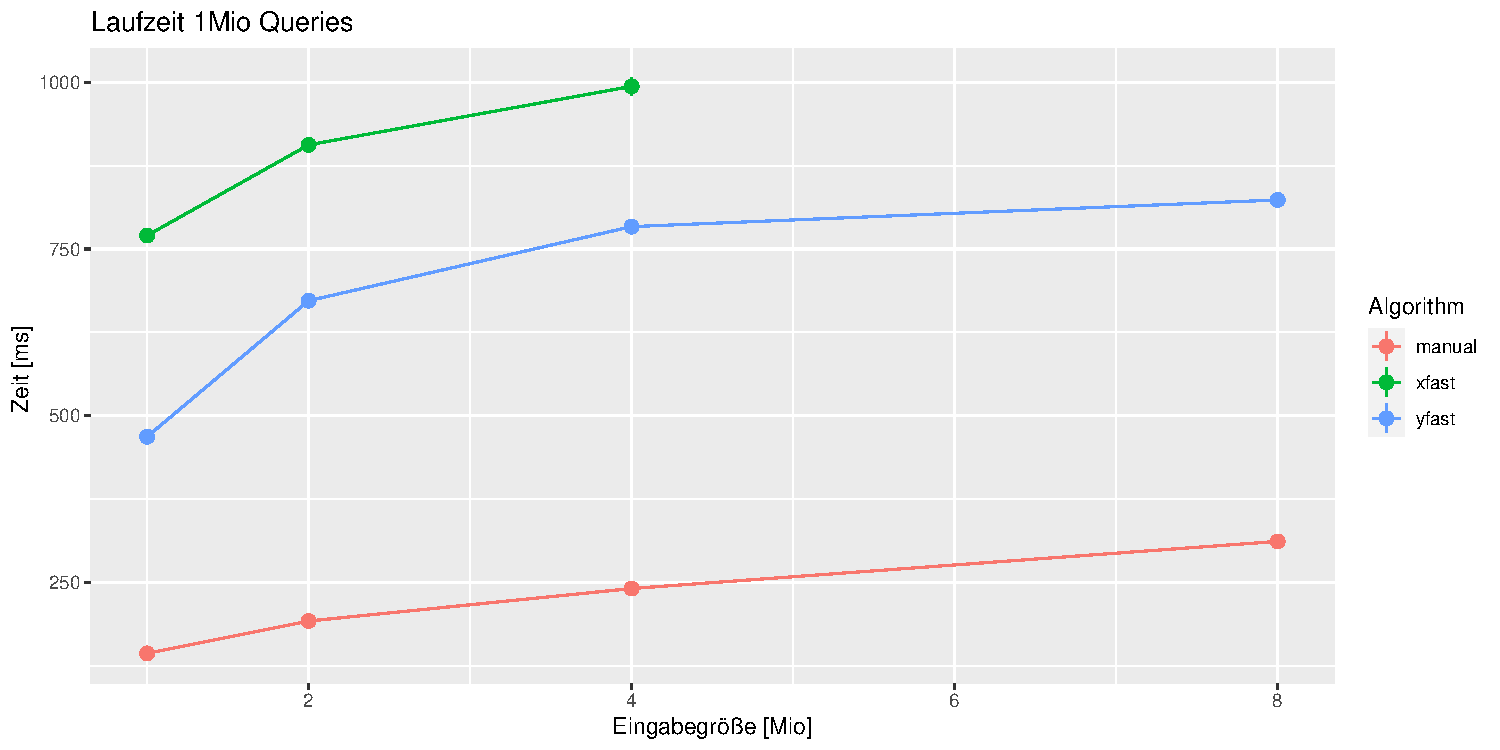
\includegraphics[page=1, width=0.9\linewidth]{../../eval/plots.pdf}
 \endminipage\hfill
 \minipage{0.5\textwidth}%
 \centering
\includegraphics[page=4, width=0.9\linewidth]{../../eval/plots.pdf}
 \endminipage
 \caption{RMQ: Running times}
  \label{fig:rmq_rt_init}
\end{figure}
 
Figure~\ref{fig:rmq_rt_init} shows the runtime of different predecessor data structures (on the left) and 
the construction time (on the right). The "manual" algorithm corresponds to std::lower\_bound and acts as a 
baseline. As we can see data structures are significantly slower than the standard library algorithm. One 
reason for this is that for both tries I did not implement perfect hashing and instead used the 
std::unordered\_map which does not guarantee constant running time. Additionally the constant factory of my 
data structures are significantly higher than with the stl algorithm, since the data structure is 
originally designed for a dynamic use case. Another interesting part is that the queries on the y-Fast-Trie 
are a lot faster than on the x-Fast-Trie. This is most likely due to the significantly higher memory usage 
of the x-Fast-Trie, which is also why its plot stops at $n=4$ using too much memory for larger inputs.

\begin{figure}[!htb]
 \minipage{0.5\textwidth}
 \centering
\includegraphics[page=6, width=0.9\linewidth]{../../eval/plots.pdf}
 \endminipage\hfill
 \minipage{0.5\textwidth}%
 \centering
\includegraphics[page=8, width=0.9\linewidth]{../../eval/plots.pdf}
 \endminipage
 \caption{RMQ: Memory usage}
  \label{fig:rmq_mem}
\end{figure}
 
Figure~\ref{fig:rmq_mem} shows memory usage relative to $n$ (left) and relative to the largest input 
(right). As we can see, the y-Fast-Trie improves memory usage dramatically, which is in accordance with 
theory since we loose the height of the tree $W$ as a factor. We can also see the effect of dynamically 
determinating the height of the Tree on the right. Since for smaller numbers the tree needs to be less high 
we can also reduce memory consumption accordingly. The x-Fast-Trie is missing in the right plot since it is 
done on instances with eight million inputs, for which it consumes too much memory.

\begin{figure}[!htb]
 \minipage{0.5\textwidth}
 \centering
\includegraphics[page=9, width=0.9\linewidth]{../../eval/plots.pdf}
 \endminipage\hfill
 \minipage{0.5\textwidth}%
 \centering
\includegraphics[page=10, width=0.9\linewidth]{../../eval/plots.pdf}
 \endminipage
 \linebreak
 \minipage{0.5\textwidth}%
 \centering
\includegraphics[page=13, width=0.9\linewidth]{../../eval/plots.pdf}
 \endminipage
   \caption{PD: Running Time and Memory Usage}
      \label{fig:pd}
\end{figure}

Figure~\ref{fig:pd} shows the results for the range minimum queries. Unfortunately there is no baseline to 
compare to since the naive data structure consumes way too much memory and a baseline algorithm like 
std::min\_element is extremely slow for any appropriately large input. As expected the queries on the 
linear data-structure are approximately 3 to 4 times slower than on the nlogn data structure, since the 
linear one not only has to do a query on the nlogn but also up to two additionally partial queries. 
Determining which queries to do requires some branching which could also be a factor in the slower running 
time. On the other hand we can clearly see the benefits of the smaller memory footprint of the linear data 
structure resulting in smaller construction time (top right) and significantly less memory usage per 
input (bottom).
%%
%% Bibliography
%%

%% Please use bibtex, 

\bibliography{lipics-v2021-sample-article}

\appendix

\end{document}
